\section{Background Information}


\subsection{Kinect}

\subsubsection{Overview}
The Kinect was developed and launched in 2010 by Microsoft. At the time of its release, it revolutionised depth acquisition technology as it was the first depth sensing device that was available to the consumer market. This low-cost, freely available technology made depth sensing accessible and caused an explosion in the use of of depth data for various applications. \cite{kinectComp2011}

\subsubsection{Versions}

\paragraph{Kinect for Xbox 360}
The first generation Kinect was launched in 2010. It was released for the Xbox 360 gaming console. It is officially called the Kinect for Xbox 360. \cite{kinectComp2011} A picture can be seen in Figure \ref{fig:kinect360}. However, it is referred to by various names in different literature. Below are different names used to refer to the Kinect for Xbox 360:

\begin{figure}[ht]
	\centering
	{%
		\setlength{\fboxsep}{0pt}%
		\setlength{\fboxrule}{0.5pt}%
		\fbox{
			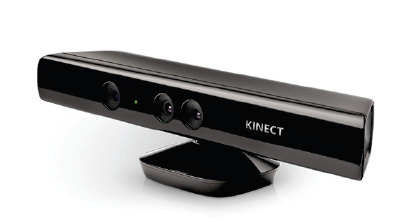
\includegraphics[width=0.7\textwidth]{Kinect360.png}
	}}
	\caption{Kinect for Xbox 360 \cite{kinectComp2011}}
	\label{fig:kinect360}
\end{figure}

\begin{itemize}
	\item First Generation Kinect 
	\item Kinect Version 1 (v1)
	\item Xbox Kinect 360 
\end{itemize} 

\paragraph{Kinect for Xbox One}
The second generation Kinect was launched in 2013. It was released with the Xbox One gaming console and is, thus, officially called the Kinect for Xbox One. \cite{kinectComp2011} A picture can be seen in Figure \ref{fig:kinectOne}. It is also referred to by different names, which are listed below for completeness:

\begin{figure}[ht]
	\centering
	{%
		\setlength{\fboxsep}{0pt}%
		\setlength{\fboxrule}{0.5pt}%
		\fbox{
			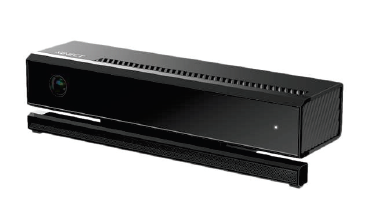
\includegraphics[width=0.7\textwidth]{KinectOne.png}
	}}
	\caption{Kinect for Xbox One \cite{kinectComp2011}}
	\label{fig:kinectOne}
\end{figure}

\begin{itemize}
	\item Second Generation Kinect 
	\item Kinect Version 2 (v2)
	\item Xbox Kinect One 
\end{itemize} 

\paragraph{Kinect for Windows}
For each generation of Kinect for Xbox released, a Kinect for Windows was released. The version numbers correlate (I.e. The Kinect for Windows also has a v1 and v2). Kinect for Windows was created to be used by a computer whereas the Kinect for Xbox to be used by the console. They are, however, functionally identical and thus, a Kinect for Xbox can be "converted" to a  Kinect for Windows by using a USB adapter. The only difference with this is that the Kinect for Windows supports "Near Mode" whereas a Kinect for Xbox used with an adapter does not. ("Near Mode" will be explained further in Section \hl{(Near Mode explanation)})

\paragraph{Kinect Used}
In this project, the Kinect for Xbox 360 with a USB adapter was used for development. Further reasons for this component choice is given in Section \hl{(Component Selection)}

\subsubsection{Components and Specifications}
The Kinect for Windows (Kinect for Xbox 360 with a USB adapter) consists of a stand and a housing for the sensing components. Between the housing and a stand is a motor that is able to adjust the vertical tilt of the housing. The Kinect is able to achieve a maximum viewing angle of $43^{\circ}$ vertical by $57^{\circ}$ horizontal. It also has a vertical tilt range of $\pm27^{\circ}$. \cite{msdnKinectSpecs2017}

The housing contains the following main components:

\begin{itemize}
	\item An RGB Camera or Colour Sensor
	\item An IR Emitter
	\item An IR Depth Sensor
	\item A Microphone Array
	\item A 3-axis Accelerometer
\end{itemize}

The configuration of the stand, housing and internal components can be seen in Figure \ref{fig:kinectComponents}. A more detailed explanation of each of the components necessary for this project is included below:

\begin{figure}[ht]
	\centering
	{%
		\setlength{\fboxsep}{0pt}%
		\setlength{\fboxrule}{0.5pt}%
		\fbox{
			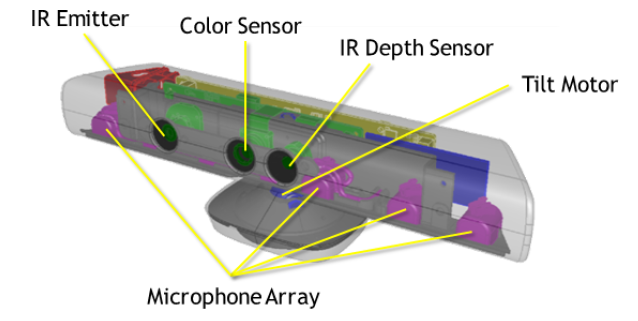
\includegraphics[width=0.7\textwidth]{Kinect360Components.png}
	}}
	\caption{Internal component layout of the Kinect for Xbox 360 \cite{msdnKinectSpecs2017}}
	\label{fig:kinectComponents}
\end{figure}

\paragraph{Colour Sensor}

\paragraph{title}

Depth, RGB and IR Sensors

\subsubsection{Extension on Depth Camera}

\subsubsection{Spaces}
Conversion to 3D space \cite{nonContact2017}\\

\paragraph{3D Points - No calibration}

\subsubsection{Internal Process}
Middleware \cite{nonContact2017}\\
Joint Filtering\\

\subsubsection{Skeleton Tracking}
Skeleton tracking\\
Known errors\\
Guidelines for measurements\\

\subsubsection{Noise}




\subsection{Microsoft SDK}

\subsubsection{Digital Information}

\subsubsection{Kinect Toolkit}

\paragraph{BackgroundRemoval Class}

\paragraph{Colour, Depth Class}


\subsection{Measurement}

\subsubsection{Pythagoras}
3D distance \cite{nonContact2017}\\

\subsubsection{Accuracy}
Error formula \cite{nonContact2017}\\

\subsection{Modelling}

\subsubsection{Ellipse}


\subsection{Augmented Reality}


\subsection{Accuracy/Other Improvement }